
\documentclass{article}
\usepackage[headheight=20pt, margin=1.0in, top=1.2in]{geometry}
\usepackage{amsmath, amssymb, amsthm, thmtools, tcolorbox, array, graphicx, makeidx, cancel, multirow, fancyhdr, xypic, color, nicefrac, rotating, multicol, caption, subcaption, xcolor, tikz, tikz-3dplot, tikz-cd, pgfplots, import, enumitem, calc, booktabs, wrapfig, siunitx, hyperref,float}
\hypersetup{colorlinks=true,linkcolor=blue}
\usepackage[all]{xy}
\usepackage{esint}
\setlength{\parindent}{0in}
\sisetup{per-mode = symbol}
\usetikzlibrary{calc,arrows,svg.path,decorations.markings,patterns,matrix,3d,fit}
\usepgfplotslibrary{groupplots}
\pgfplotsset{compat=newest}
\newtcolorbox{mydefbox}[2][]{colback=red!5!white,colframe=red!75!black,fonttitle=\bfseries,title=#2,#1}
\newtcolorbox{mythmbox}[2][]{colback=gray!5!white,colframe=gray!75!black,fonttitle=\bfseries,title=#2,#1}
\newtcolorbox{myexamplebox}[2][]{colback=green!5!white,colframe=green!75!black,fonttitle=\bfseries,title=#2,#1}
\newtcolorbox{mypropbox}[2][]{colback=blue!5!white,colframe=blue!75!black,fonttitle=\bfseries,title=#2,#1}
\declaretheoremstyle[headfont=\color{blue}\normalfont\bfseries,]{colored}
\theoremstyle{definition}
\newtheorem{theorem}{Theorem}
\newtheorem{corollary}[theorem]{Corollary}
\newtheorem{lemma}[theorem]{Lemma}
\newtheorem{proposition}[theorem]{Proposition}
\newtheorem{problem}[theorem]{Problem}
\newtheorem{definition}[theorem]{Definition}
\newtheorem{exercise}[theorem]{Exercise}
\newtheorem{example}[theorem]{Example}
\newtheorem{solution}[theorem]{Solution}
\newtheorem*{thm}{Theorem}
\newtheorem*{lem}{Lemma}
\newtheorem*{prob}{Problem}
\newtheorem*{exer}{Exercise}
\newtheorem*{prop}{Proposition}
\def\R{\mathbb{R}}
\def\F{\mathbb{F}}
\def\Q{\mathbb{Q}}
\def\C{\mathbb{C}}
\def\N{\mathbb{N}}
\def\Z{\mathbb{Z}}
\def\Ra{\Rightarrow}
\def\e{\epsilon}
\newcommand{\typo}[1]{{\color{red}{#1}}}
\newcommand\thedate{\today}
\newcommand{\mb}{\textbf}
\newcommand{\norm}[2]{\|{#1}\|_{#2}}
\newcommand{\normm}[1]{\|#1\|}
\newcommand{\mat}[1]{\begin{bmatrix} #1 \end{bmatrix}}
\newcommand{\eqtext}[1]{\hspace{3mm} \text{#1} \hspace{3mm}}
\newcommand{\set}[1]{\{#1\}}
\newcommand{\inte}{\textrm{int}}
\newcommand{\ra}{\rightarrow}
\newcommand{\minv}{^{-1}}
\newcommand{\tx}[1]{\text{ {#1} }}
\newcommand{\abs}[1]{|#1|}
\newcommand{\mc}[1]{\mathcal{#1}}
\newcommand{\uniflim}{\mathop{\mathrm{unif\lim}}}
\newcommand{\notimplies}{\mathrel{{\ooalign{\hidewidth$\not\phantom{=}$\hidewidth\cr$\implies$}}}}
\pagestyle{fancy}
\fancyhf{}
\fancyhead[L]{Title of the Document}
\fancyhead[C]{}
\fancyhead[R]{\thepage}
\fancyfoot[L]{}
\fancyfoot[C]{}
\fancyfoot[R]{}
\renewcommand{\headrulewidth}{0.4pt}
\renewcommand{\footrulewidth}{0.4pt}
\numberwithin{equation}{section}
% Increase spacing between paragraphs
\setlength{\parskip}{1em}
% Increase spacing before and after sections
\usepackage{titlesec}
\titlespacing*{\section}{0pt}{3ex plus 1ex minus .2ex}{2ex plus .2ex}
\titlespacing*{\subsection}{0pt}{2ex plus 1ex minus .2ex}{1ex plus .2ex}
\titlespacing*{\subsubsection}{0pt}{1ex plus 1ex minus .2ex}{1ex plus .2ex}
\title{\textbf{Title of the Document}}
\author{Author Name}
\date{\today}
\begin{document}
\maketitle
\tableofcontents
\newpage
\section{Exercises}
\begin{enumerate}
    \item Let $(X,d)$ be a metric space and $S \subseteq X$. Show that $\overline{S}^0 \subseteq S^0 = \emptyset$.
    \item Show that for an arbitrary choice of $a,b,r \in \mathbb{R}$, the closed disk $(x-a)^2 + (y-b)^2 \leq r^2$ is a bounded set in $\mathbb{R}^2$.
    \item Let $(X,d)$ be a metric space and let $x,y \in X$. Show that if $d(x,y) < \epsilon$ for every $\epsilon > 0$, then $x = y$.
\end{enumerate}

\begin{proof}
    (i) Assume $\exists \epsilon > 0, \exists x \in \overline{S}^0, x \not\in S^0$.

    Then by $x \in \overline{S}^0$, $\exists \epsilon > 0: B_\epsilon(x) \subseteq S$. 

    However, by $x \not\in S^0$, this value of $\epsilon > 0$ implies $B_{\epsilon / 2}(x) \cap S^c \neq \emptyset$ $\Rightarrow B_{\epsilon / 2}(x) \not\subseteq S$, which is a contradiction.

    This implies our assumption that $x \in \overline{S}^0 \cap S^0$ must be false and $\overline{S}^0 \cap S^0 = \emptyset$.
\end{proof}

\begin{proof}
    (ii) A set $S$ is bounded if and only if $\exists M \in \mathbb{R}^+ \ \forall x, y \in S$, $d(x,y) < M$. 

    Let $a, b, r \in \mathbb{R}$.
    $S := \{(x,y) \in \mathbb{R} \} [(x-a)^2 + (y-b)^2 \leq r^2]$

    \begin{align*}
        &\Rightarrow x^2 - 2ax + a^2 + y^2 - 2yb + b^2 \leq r^2 \\
        &\Rightarrow x^2 - 2ax + y^2 - 2yb \leq r^2 - a^2 - b^2 \\
        &\Rightarrow x^2 + y^2 \leq r^2 - a^2 - b^2 + 2ax + 2yb
    \end{align*}

    We need to show $x^2$ is bounded.
    \begin{itemize}
        \item $(x-a)^2 \leq r^2$ 
            $\Rightarrow |x - a| \leq |r|$
            $\Rightarrow |x-a| \leq |r| + |a|$
            $\Rightarrow |x| = |x-a + a| \leq |x-a| + |a| \leq r + a$
    \end{itemize}
\end{proof}

\begin{align*}
    &\begin{array}{c}
    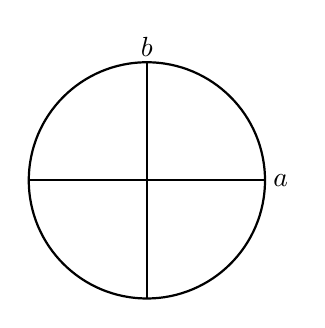
\begin{tikzpicture}
        \draw[thick] (0,0) circle (1.5cm);
        \draw[thick] (-1.5,0) -- (1.5,0);
        \draw[thick] (0,-1.5) -- (0,1.5);
        \node at (1.7,0) {$a$};
        \node at (0,1.7) {$b$};
    \end{tikzpicture}
    \end{array}
    \Rightarrow |y| \leq r + |a| \\
    &\Rightarrow \ x^2 \leq (r + |a|)^2
\end{align*}

\text{Same for $y$,} \quad y^2 \leq (r + |b|)^2

\forall z = (x,y) \in D^2_{a,b}

\|z\| = \sqrt{x^2 + y^2}
\leq \sqrt{(r + |a|)^2 + (r + |b|)^2}

\text{Thus, if} \quad M = \sqrt{(r + |a|)^2 + (r + |b|)^2}, \quad \text{the bound holds.}

\text{\# IS boundedness = distance boundedness:}

\text{Let} \quad x = (x_1, x_2), \quad y = (y_1, y_2) \in D^2_{a,b}, \quad z \in \{x,y\}

(x_2 - a)^2 + (x_2 - b)^2 = r^2
\Rightarrow d(z, (a,b)) = \sqrt{(z_1 - a)^2 + (z_2 - b)^2} \leq r

\Rightarrow d(x,y) \leq d(x, (a,b)) + d(y, (a,b))
= \sqrt{(x_1 - a)^2 + (x_2 - b)^2} + \sqrt{(y_1 - a)^2 + (y_2 - b)^2}
\leq r + r = 2r.

\begin{itemize}
    \item[(iii)] Suppose that \(x \neq y\). Then \(d(x,y) \neq 0\). Thus if we choose \(\varepsilon = d(x,y) \implies \varepsilon > 0\) but \(d(x,y) \notin \varepsilon\). (contradiction).
\end{itemize}

\begin{itemize}
    \item[(contradiction)] Suppose \(x \neq y\) and so \(d(x,y) \neq 0\). Choose \(\varepsilon > 0\) so that \(\varepsilon = d(x,y)\). Then we must have \(d(x,y) \leq \varepsilon = d(\frac{x+y}{2})\), which is a contradiction, as this implies if \(d(x,y) > 0\) then \(d(x,y) = \epsilon = \frac{\epsilon}{2}\). Thus,

    $
    \epsilon > 2 \frac{\epsilon}{2} \implies 2 \epsilon \leq \epsilon
    $

    Thus, \(x = y\).
\end{itemize}

\begin{itemize}
    \item[(iv)] Let \((V, \| \cdot \|)\) be a normed vector space. Then let \(r > 0\) and \(x \in V\). Then

    $
    B_r(x) = \{ u \in V | d(x,u) < r \}
    $

    $
    B_{\epsilon + \|u\|}(0) = \{ v \in V | d(0,u) < r + \| u \| \}
    $

    $
    \text{Let } y \in B_r(x) \implies d(o,y) \leq d(o,x) + d(x,y)
    $

    $
    \leq \| x \| + r \implies B_r(x) \subseteq B_{r + \| x \|}(0)
    $

    \begin{center}
        \includegraphics{circle_drawing.png}
    \end{center}
\end{itemize}

\begin{itemize}
    \item[(v)] Suppose \(S\) is bounded. Then \(\exists M \in \mathbb{R} > 0: \forall x \in S \| x \| \leq M\).

    $
    \text{(Equivalent to } \exists M \in \mathbb{R}: \forall x \in V) x \in B_{M}(0)
    $
\end{itemize}\end{document}